\def\pctreegraphmatrix{%
  \begin{tabular}[b]
    {>{\columncolor{\tblhcolor}} l llllllll|}
    \hline
    $r_1$   &\un &0   &\un &0   &0   &0    &0   &0   \\
    $r_2$   &\un &\un &0   &0   &0   &0    &0   &0   \\
    $r_3$   &0   &\un &\un &0   &0   &0    &0   &0   \\
    $r_4$   &0   &0   &\un &\un &0   &0    &0   &0   \\
    $r_5$   &0   &0   &\un &\un &\un &0    &0   &0   \\
    $r_6$   &0   &0   &\un &0   &\un &0    &0   &0   \\
    $r_7$   &0   &0   &\un &0   &0   &\un  &0   &0   \\
    $r_8$   &0   &0   &\un &0   &0   &\un  &\un &0   \\
    $r_9$   &0   &0   &\un &0   &0   &0    &\un &0   \\
    $r_{10}$ &0   &0   &\un &0   &0   &0    &0   &\un \\
    \hline
  \end{tabular}
}%

\def\pctreegraphii{%
 \begin{tikzpicture}
    [grow cyclic, 
     level 1/.style={level distance=7mm,sibling angle=100}, 
     level 2/.style={level distance=10mm, sibling angle=35}
     ]
    \node[circle,inner sep=3pt,fill]{}%
      child{node[circle,draw,inner sep=0pt,double, double
        distance=1pt]{\ \ \ }%    
        child{node{$r_9$}}%
        child{node{$r_8$}}%
        child{node{$r_7$}}%
      }%
      child{node[circle,draw,inner sep=0pt,double, double
        distance=1pt](p456){\ \ \ }%
        child{node(r4){$r_4$}}%
        child{node(r5){$r_5$}}%
        child{node(r6){$r_6$}}%
      }%
      child{node[circle,draw,inner sep=0pt,double, double
        distance=1pt]{\ \ \ }%  
        child{node{$r_3$}}%
        child{node{$r_2$}}%
        child{node{$r_1$}}%
      }%
      child[level distance=10mm]{ node{$r_{10}$}}%
     ;%

     \begin{pgfonlayer}{background}
       \node[rectangle, rounded corners=10pt,%
            inner sep=2pt, fill=red!30,%
            opacity=0.5,% 
            fit = (p456)(r4) (r5) (r6)] (flipped){};%
     \end{pgfonlayer}    
  \end{tikzpicture}
}%


\def\pctreegraphi{%
 \begin{tikzpicture}
    [grow cyclic, 
     level 1/.style={level distance=7mm,sibling angle=100}, 
     level 2/.style={level distance=10mm, sibling angle=35}
     ]
    \node[circle,inner sep=3pt,fill]{}%
      child{node[circle,draw,inner sep=0pt,double, double
        distance=1pt]{\ \ \ }%    
        child{node{$r_9$}}%
        child{node{$r_8$}}%
        child{node{$r_7$}}%
      }%
      child{node[circle,draw,inner sep=0pt,double, double
        distance=1pt](p456){\ \ \ }%
        child{node(r6){$r_6$}}%
        child{node(r5){$r_5$}}%
        child{node(r4){$r_4$}}%
      }%
      child{node[circle,draw,inner sep=0pt,double, double
        distance=1pt]{\ \ \ }%  
        child{node{$r_3$}}%
        child{node{$r_2$}}%
        child{node{$r_1$}}%
      }%
      child[level distance=10mm]{ node{$r_{10}$}}%
     ;%

     \begin{pgfonlayer}{background}
       \node[rectangle, rounded corners=10pt,%
            inner sep=2pt, fill=red!30,%
            opacity=0.5,% 
            fit = (p456)(r4) (r5) (r6)] (flipped){};%
     \end{pgfonlayer}    
  \end{tikzpicture}
}%



\def\graphici{%
  $G_1$:\\ 
  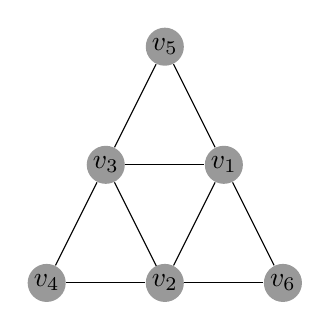
\begin{tikzpicture}[every node/.style={circle,inner
      sep=1pt,fill=gray!80}] %
    % Using tree mode of drawing to avoid coordinate coding
    \node{$v_5$}%
      child{node (v3){$v_3$}%
        child{node (v4){$v_4$}}%
        child{node {}}% DUMMY to make alignment work
      }%
      child{node (v1){$v_1$}%
        child{node (v2){$v_2$}}%
        child{node (v6){$v_6$}}%
      }%
      ;%

      \draw (v3)--(v1);%
      \draw (v2)--(v4);%     
      \draw (v2)--(v6);%
  \end{tikzpicture}
}%

%%%%%%%%%% END
\def\studygroupsI{%
  \begin{tikzpicture}


%    \draw[help lines] (0,0) grid (3,4);%

    \draw[scale=1.5,
          every node/.style={draw = none,%
                             rectangle,rounded corners,%
                             fill=gray!60,%
                             inner sep=3pt}]%

      (0,0) node(sn){\xSn}%
      (0,1) node(wo){\xWo}%
      (2,3) node(sa){\xSa}%
      (1,1) node(pi){\xPi}%
      (3,2) node(fr){\xFr}%
      (2,2) node(ch){\xCh}%
      (2,1) node(vi){\xVi}%
      (1,2) node(pa){\xPa}%

      (2,4) node(lu){\xLu}%
      (3,1) node(li){\xLi}%
      (3,3) node(sc){\xSc}%
      ;%

    \begin{pgfonlayer}{background}
      \begin{scope}[every node/.style={ellipse,%
%                                       rounded corners=5pt,%
                                       inner sep=2pt,%
                                       draw,%=black,%
                                       opacity=0.5%
                                     }]%

      \node[fill=orange!30, fit = (sn) (wo) (pi)]{}; %%
      \node[fill=blue!30, fit = (pi) (vi) (pa) (ch)]{}; %%
      \node[fill=green!30, fit = (fr) (vi) (li) (ch)]{}; %%      
      \node[fill=red!30, fit = (fr) (sc) (sa) (lu) (ch)]{}; %%
      \end{scope}
    \end{pgfonlayer}

  \end{tikzpicture}
}%

\def\studygroupsIII{%
  \begin{tikzpicture}
%    \draw[help lines] (0,0) grid (3,4);%

    \draw[scale=1.5,
          every node/.style={draw = none,%
                             rectangle,rounded corners,%
                             fill=gray!60,%
                             inner sep=3pt}]%

      (2,3) node(sa){\xSa}%
      (1,1) node(pi){\xPi}%
      (3,2) node(fr){\xFr}%
      (2,2) node(ch){\xCh}%
      (2,1) node(vi){\xVi}%

      ;%

    \begin{pgfonlayer}{background}
      \begin{scope}[every node/.style={ellipse,%
%                                       rounded corners=5pt,%
                                       inner sep=2pt,%
                                       draw,%=black,%
                                       opacity=0.5%
                                     }]%

      \node[fill=blue!30, fit = (pi) (vi) (ch)]{}; %%
      \node[fill=green!30, fit = (fr) (vi) (ch)]{}; %%      
      \node[fill=red!30, fit = (fr) (sa) (ch)]{}; %%
      \node[fill=orange!30, fit = (pi)]{}; %%
      \end{scope}
    \end{pgfonlayer}

  \end{tikzpicture}
}%

\def\studygroupsIVa{%
  \begin{tikzpicture}
%    \draw[help lines] (0,0) grid (3,4);%

    \draw[scale=1.5,
          every node/.style={draw = none,%
                             rectangle,rounded corners,%
                             fill=gray!60,%
                             inner sep=3pt}]%

      (2,3) node(sa){\xSa}%
      (1,1) node(pi){\xPi}%
      (3,2) node(fr){\xFr}%
      (2,2) node(ch){\xCh}%
      (2,1) node(vi){\xVi}%

      ;%

    \begin{pgfonlayer}{background}
      \begin{scope}[every node/.style={ellipse,%
%                                       rounded corners=5pt,%
                                       inner sep=2pt,%
                                       draw,%=black,%
                                       opacity=0.5%
                                     }]%

      \node[fill=green!30, fit = (fr) (vi) (ch)]{}; %%      
      \node[fill=red!30, fit = (fr) (sa) (ch)]{}; %%
      \node[fill=orange!30, fit = (pi)]{}; %%
      \node[fill=blue!30, fit = (vi) (ch)]{}; %%
      \end{scope}
    \end{pgfonlayer}

  \end{tikzpicture}
}%

\def\studygroupsIVb{%
  \begin{tikzpicture}
%    \draw[help lines] (0,0) grid (3,4);%

    \draw[scale=1.5,
          every node/.style={draw = none,%
                             rectangle,rounded corners,%
                             fill=gray!60,%
                             inner sep=3pt}]%

      (2,3) node(sa){\xSa}%
      (1,1) node(pi){\xPi}%
      (3,2) node(fr){\xFr}%
      (2,2) node(ch){\xCh}%
      (2,1) node(vi){\xVi}%

      ;%

    \begin{pgfonlayer}{background}
      \begin{scope}[every node/.style={ellipse,%
%                                       rounded corners=5pt,%
                                       inner sep=2pt,%
                                       draw,%=black,%
                                       opacity=0.5%
                                     }]%

     \node[fill=green!80, fit = (fr) (ch)]{}; %%

      \node[fill=red!30, fit = (sa)]{}; %%

      \node[fill=orange!30, fit = (pi)]{}; %%
      \node[fill=blue!30, fit = (vi) (ch)]{}; %%
      \node[fill=green!30, fit = (vi)]{}; %%      
      \end{scope}
    \end{pgfonlayer}

  \end{tikzpicture}
}%

\def\studygroupsVI{%
  \begin{tikzpicture}
%    \draw[help lines] (0,0) grid (3,4);%

    \draw[scale=1.5,
          every node/.style={draw = none,%
                             rectangle,rounded corners,%
                             fill=gray!60,%
                             inner sep=3pt}]%

      (2,2) node(ch){\xCh}%
      (2,1) node(vi){\xVi}%

      ;%

    \begin{pgfonlayer}{background}
      \begin{scope}[every node/.style={ellipse,%
%                                       rounded corners=5pt,%
                                       inner sep=2pt,%
                                       draw,%=black,%
                                       opacity=0.5%
                                     }]%

     \node[fill=green!80, fit = (ch)]{}; %%
      \node[fill=blue!30, fit = (vi) (ch)]{}; %%
      \node[fill=green!30, fit = (vi)]{}; %%      
      \end{scope}
    \end{pgfonlayer}

  \end{tikzpicture}
}%



\def\infiniteloopI{%
  \begin{tikzpicture}[every node/.style={circle,inner sep=2pt,draw=gray!90}]%

%    \draw[help lines] (-1,0) grid (6,5);%

    \draw%
      (0,2) node(a7){7} %
      (1,2) node(a2){2} %
      (2,2) node(a6){6} %
      (3,2) node(a5){5} %
      (4,2) node(a3){3} %
      (5,2) node(a11){11} %
      (1,1) node(a4){4} %
      (1,3) node(a8){8} %
      (2,1) node(a10){10} %      
      (3,3) node(a1){1} %
      (3,4) node(a9){9} %
     ;%

    \draw[very thick]%
      (a2) -- (a4)%
      (a2) -- (a8)%
      (a5) -- (a1) -- (a9)
      (a6) -- (a10)
      (a7) --
      (a2) --%
      (a6) --%
      (a5) --%
      (a3) --%
      (a11) %
      ;%

    \begin{pgfonlayer}{background}
    \node[rectangle, rounded corners=5pt, inner sep=6pt,%
      fill=green!30,  opacity=0.5, fit = (a10) (a6) (a5) (a3)]{}; %%
    \node[rectangle, rounded corners=5pt, %
      fill=orange!30, opacity=0.5, fit = (a4) (a2) (a8)]{}; %%
    \node[rectangle, rounded corners=5pt, %
      fill=red!30,    opacity=0.5, fit = (a9) (a1) (a5) (a3) (a11)]{}; %%
    \node[rectangle, rounded corners=5pt, %
      fill=blue!30,   opacity=0.5, fit = (a7) (a2) (a6) (a5)]{}; %%

   \end{pgfonlayer}
  \end{tikzpicture}
}%

\def\infiniteloopIII{%
  \begin{tikzpicture}[every node/.style={circle,inner sep=2pt,draw=gray!90}]%

    % \draw[help lines] (-1,0) grid (6,5);%
    
    % Tree nodes/apartments
    \draw%
      (0,2) node(a7){7} %
      (1,2) node(a2){2} %
      (2,2) node(a6){6} %
      (3,2) node(a5){5} %
      (4,2) node(a3){3} %
      (5,2) node(a11){11} %
      (1,1) node(a4){4} %
      (1,3) node(a8){8} %
      (2,1) node(a10){10} %      
      (3,3) node(a1){1} %
      (3,4) node(a9){9} %
     ;%

    % Tree
    \draw[very thick]%
      (a5) -- (a1)
      (a2) --%
      (a6) --%
      (a5) --%
      (a3) %
      ;%

    % Pruned leaves
    \draw [thin,densely dotted]% 
      (a7) -- (a2)%
      (a2) -- (a8)%
      (a2) -- (a4)%
      (a6) -- (a10)%
      (a3) -- (a11)%
      (a1) -- (a9)%
      ;%

    % Routes
    \begin{pgfonlayer}{background}
      \begin{scope}[every node/.style={rectangle,%
                                       rounded corners=5pt,%
                                       inner sep=2pt,%
                                       draw=black,%
                                       opacity=0.5%
                                     }]%

      \node[fill=green!30, fit = (a6) (a5) (a3), inner sep=6pt]{}; %%
      \node[fill=red!30,   fit = (a1) (a5) (a3) ,inner sep=4pt]{}; %%
      \node[fill=orange!30,fit = (a2) ,inner sep=4pt]{}; %%
      \node[fill=blue!30,  fit = (a2) (a6) (a5)]{}; %%
     \end{scope}
    \end{pgfonlayer}

   % Assigned leaf nodes/ allocated apartments
    \draw[every node/.style={draw = none,%
                             rectangle,rounded corners,%
                             fill=gray!50,%
                             inner sep=3pt}]%

      (a7)  node[left=10pt=10pt] {\xPa} %
      (a11) node[right=10pt] {\xSc} %
      (a4)  node[below=10pt] {\xWo} %
      (a8)  node[above=10pt] {\xSn} %
      (a10) node[below=10pt] {\xLi} %      
      (a9)  node[above=10pt] {\xLu} %
     ;%

  \end{tikzpicture}
}%

\def\infiniteloopIVa{%
  \begin{tikzpicture}[every node/.style={circle,inner sep=2pt,draw=gray!90}]%

    % \draw[help lines] (-1,0) grid (6,5);%
    
    % Tree nodes/apartments
    \draw%
      (1,2) node(a2){2} %
      (2,2) node(a6){6} %
      (3,2) node(a5){5} %
      (4,2) node(a3){3} %
      (3,3) node(a1){1} %
     ;%

    % Tree
    \draw[very thick]%
      (a5) -- (a1)
      (a2) --%
      (a6) --%
      (a5) --%
      (a3) %
      ;%

    % Pruned leaves
    \draw [thin,densely dotted]% 
     ;%

    % Routes
    \begin{pgfonlayer}{background}
      \begin{scope}[every node/.style={rectangle,%
                                       rounded corners=5pt,%
                                       inner sep=2pt,%
                                       draw=black,%
                                       opacity=0.5%
                                     }]%

      \node[fill=green!30, fit = (a6) (a5) (a3), inner sep=6pt]{}; %%
      \node[fill=red!30,   fit = (a1) (a5) (a3) ,inner sep=4pt]{}; %%
      \node[fill=blue!30,  fit = (a6) (a5)]{}; %%
      \node[fill=orange!30,fit = (a2) ,inner sep=4pt]{}; %%
      \end{scope}
    \end{pgfonlayer}

   % Assigned leaf nodes/ allocated apartments
    \draw[every node/.style={draw = none,%
                             rectangle,rounded corners,%
                             fill=gray!50,%
                             inner sep=3pt}]%

    ;%

  \end{tikzpicture}
}%

\def\infiniteloopIVb{%
  \begin{tikzpicture}[every node/.style={circle,inner sep=2pt,draw=gray!90}]%

    % \draw[help lines] (-1,0) grid (6,5);%
    
    % Tree nodes/apartments
    \draw%
      (1,2) node(a2){2} %
      (2,2) node(a6){6} %
      (3,2) node(a5){5} %
      (4,2) node(a3){3} %
      (3,3) node(a1){1} %
     ;%

    % Tree
    \draw[very thick]%
      (a5) -- (a1)
      (a2) --%
      (a6) --%
      (a5) --%
      (a3) %
      ;%

    % Pruned leaves
    \draw [thin,densely dotted]% 
     ;%

    % Routes
    \begin{pgfonlayer}{background}
      \begin{scope}[every node/.style={rectangle,%
                                       rounded corners=5pt,%
                                       inner sep=2pt,%
                                       draw=black,%
                                       opacity=0.5%
                                     }]%

      \node[fill=green!30, fit = (a6)     , inner sep=6pt]{}; %%
      \node[fill=green!80, fit = (a5) (a3), inner sep=4pt]{}; %%
      \node[fill=red!30,   fit = (a1)     , inner sep=4pt]{}; %%
      \node[fill=blue!30,  fit = (a6) (a5)]{}; %%
      \node[fill=orange!30,fit = (a2)     ,inner sep=4pt]{}; %%
      \end{scope}
    \end{pgfonlayer}

   % Assigned leaf nodes/ allocated apartments
    \draw[every node/.style={draw = none,%
                             rectangle,rounded corners,%
                             fill=gray!50,%
                             inner sep=3pt}]%

    ;%

  \end{tikzpicture}
}%

\def\infiniteloopVI{%
  \begin{tikzpicture}[every node/.style={circle,inner sep=2pt,draw=gray!90}]%

    % \draw[help lines] (-1,0) grid (6,5);%
    
    % Tree nodes/apartments
    \draw%
      (1,2) node(a2){2} %
      (2,2) node(a6){6} %
      (3,2) node(a5){5} %
      (4,2) node(a3){3} %
      (3,3) node(a1){1} %
     ;%

    % Tree
    \draw[very thick]%
      (a6) -- (a5)
      ;%

    % Pruned leaves
    \draw [thin,densely dotted]% 
      (a5) -- (a1)%
      (a2) -- (a6)%
      (a5) -- (a3)%
     ;%

    % Routes
    \begin{pgfonlayer}{background}
      \begin{scope}[every node/.style={rectangle,%
                                       rounded corners=5pt,%
                                       inner sep=2pt,%
                                       draw=black,%
                                       opacity=0.5%
                                     }]%

      \node[fill=blue!30,  fit = (a6) (a5) , inner sep=6pt]{}; %%
      \node[fill=green!30, fit = (a6)     ]{}; %%
      \node[fill=green!80, fit = (a5)]{}; %%
     \end{scope}
    \end{pgfonlayer}

   % Assigned leaf nodes/ allocated apartments
    \draw[every node/.style={draw = none,%
                             rectangle,rounded corners,%
                             fill=gray!50,%
                             inner sep=3pt}]%

      (a1)  node[above=10pt] {\xSa} %
      (a2) node[left=10pt] {\xPi} %
      (a3)  node[right=10pt] {\xFr} %
    ;%

  \end{tikzpicture}
}%

\def\infiniteloopVII{%
  \begin{tikzpicture}[every node/.style={circle,inner sep=2pt,draw=gray!90}]%

    % \draw[help lines] (-1,0) grid (6,5);%
    
    % Tree nodes/apartments
    \draw%
      (2,2) node(a6){6} %
      (3,2) node(a5){5} %
     ;%

    % Tree
    \draw[very thick]%
      (a6) -- (a5)
      ;%

    % Pruned leaves
    \draw [thin,densely dotted]% 
     ;%

    % Routes
    \begin{pgfonlayer}{background}
      \begin{scope}[every node/.style={rectangle,%
                                       rounded corners=5pt,%
                                       inner sep=2pt,%
                                       draw=black,%
                                       opacity=0.5%
                                     }]%

%      \node[fill=blue!30,  fit = (a6) (a5) , inner sep=6pt]{}; %%
      \node[fill=green!30, fit = (a6)     ]{}; %%
      \node[fill=green!80, fit = (a5)]{}; %%
      \end{scope}
    \end{pgfonlayer}

   % Assigned leaf nodes/ allocated apartments
    \draw[every node/.style={draw = none,%
                             rectangle,rounded corners,%
                             fill=gray!50,%
                             inner sep=3pt}]%


      (a6) node[left=13pt] {\xVi} %
      (a5)  node[right=13pt] {\xCh} %
     ;%

  \end{tikzpicture}
}%

\def\infiniteloopVIII{%
  \begin{tikzpicture}[every node/.style={circle,inner sep=2pt,draw=gray!90}]%

%   \draw[help lines] (-1,0) grid (6,5);%

    \draw[scale=1.5]%
      (0,2) node(a7){7} %
      (1,2) node(a2){2} %
      (2,2) node(a6){6} %
      (3,2) node(a5){5} %
      (4,2) node(a3){3} %
      (5,2) node(a11){11} %
      (1,1) node(a4){4} %
      (1,3) node(a8){8} %
      (2,1) node(a10){10} %      
      (3,3) node(a1){1} %
      (3,4) node(a9){9} %
     ;%

    \draw[very thick]%
      (a2) -- (a4)%
      (a2) -- (a8)%
      (a5) -- (a1) -- (a9)
      (a6) -- (a10)
      (a7) --
      (a2) --%
      (a6) --%
      (a5) --%
      (a3) --%
      (a11) %
      ;%

    \begin{pgfonlayer}{background}
    \node[rectangle, rounded corners=5pt, %
      fill=blue!30,   opacity=0.5, fit = (a7) (a2) (a6) (a5)]{}; %%
    \node[rectangle, rounded corners=5pt, inner sep=6pt,%
      fill=green!30,  opacity=0.5, fit = (a10) (a6) (a5) (a3)]{}; %%
    \node[rectangle, rounded corners=5pt, %
      fill=orange!30, opacity=0.5, fit = (a4) (a2) (a8)]{}; %%
    \node[rectangle, rounded corners=5pt, %
      fill=red!30,    opacity=0.5, fit = (a9) (a1) (a5) (a3) (a11)]{}; %%
   \end{pgfonlayer}

   % Assigned leaf nodes/ allocated apartments
    \draw[every node/.style={draw = none,%
                             rectangle,rounded corners,%
                             fill=gray!50,%
                             inner sep=3pt}]%


     (a1) node[right=13pt] {\xSa} %
     (a2) node[above left=15pt] {\xPi} %
     (a3) node[above=13pt] {\xFr} %
     (a4) node[left=13pt] {\xWo} %
     (a5) node[below=13pt] {\xCh} %
     (a6) node[above=13pt] {\xVi} %
     (a7) node[left=13pt] {\xPa} %
     (a8) node[above=13pt] {\xSn} %
     (a9) node[right=13pt] {\xLu} %
     (a10) node[right=13pt] {\xLi} %
     (a11) node[right=13pt] {\xSc} %
     ;%

  \end{tikzpicture}
}%

%%%%%%%% BEGIN


%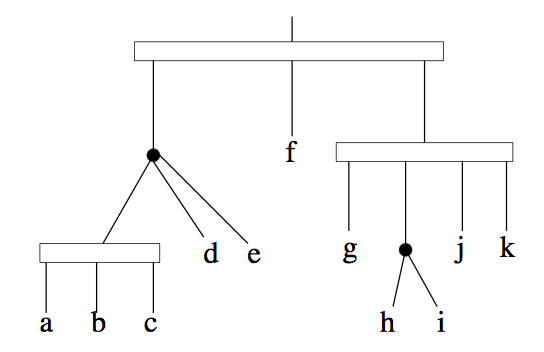
\includegraphics[scale=0.3]{../img/pqtree.png}

% 1 2 3 4 5 6 7 8 9 10 11
% a b c d e f g h i j  k

% (d,  a,  b,  c,  e,  f,  g,  h,  i,  j,     k)
% (r_4,r_1,r_2,r_3,r_5,r_6,r_7,r_8,r_9,r_{10},r_{11})

% (r_1,r_2,r_3,r_4,r_5,r_6,r_{11},r_{10},r_8,r_9,r_7)


% \pqtreegraph
% Permuting the order of the left child of the root, we see that
% $(r_4,r_1,r_2,r_3,r_5,r_6,r_7,r_8,r_9,r_{10},r_{11})$ is a \COP
% order. Reversing the order of the right child of the root, we see that
% $(r_1,r_2,r_3,r_4,r_5,r_6,r_{11},r_{10},r_8,r_9,r_7)$ is yet another
% \COP order.

